
\begin{figure*}
\parbox[][][b]{0.22\linewidth}{%
\centering 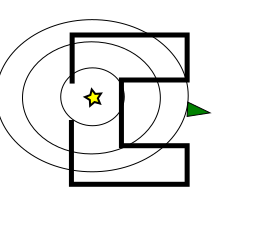
\includegraphics[width=\linewidth]{./files/media/u-maze.pdf}\\(a)}
\parbox[][][b]{0.27\linewidth}{%
\centering \includegraphics[width=\linewidth]{./files/media/deepfill-architecture.pdf}\\(b)}
\parbox[][][b]{0.24\linewidth}{%
\centering \includegraphics[width=\linewidth]{./files/media/atk_exploration.png}\\(c)}
\parbox[][][b]{0.24\linewidth}{%
\centering \includegraphics[width=\linewidth]{./files/media/zigxbee.png}\\(d)}
  \caption{
  (a) U-maze. If the green robot greedily follows the radio signal from the
  yellow target, then it is likely to get stuck in the local minima. Our
  algorithm has dual objective of exploration and source seeking. When the gain
  in source seeking is small then the robot reverts to environment exploration
  and escapes local minima.
  (b) DeepFill architecture. Image from \cite{yu2018DeepFill}
  (c) Our multi-robot team of jackal robots exploring Atkinson Hall's first floor getting measurements from ZigXbees transmitters. 
  (d) On the right a picture of the ZigXbee transmitter used on these experiments.}%
  \label{fig:exp:expl_atk}%
  \label{fig:deepfill}%
  \label{fig:c-maze}
\end{figure*}

 %
\begin{figure*}[h!]%
  \def\frac{0.24}
  \includegraphics[width=\frac\linewidth]{./files/media/department_diiga/00016_input.png}%
  \includegraphics[width=\frac\linewidth]{./files/media/department_diiga/00016_mask.png}%
  \includegraphics[width=\frac\linewidth]{./files/media/department_diiga/0016_output.png}%
  \includegraphics[width=\frac\linewidth]{./files/media/department_diiga/00016_estimated.png}%
  \\%
  \includegraphics[width=\frac\linewidth]{./files/media/fr_campus_100p_10cm/00009_input.png}%
  \includegraphics[width=\frac\linewidth]{./files/media/fr_campus_100p_10cm/00009_mask.png}%
  \includegraphics[width=\frac\linewidth]{./files/media/fr_campus_100p_10cm/00009_output.png}%
  \includegraphics[width=\frac\linewidth]{./files/media/fr_campus_100p_10cm/00009_estimated.png}%
  \caption{Map prediction using DeepFill~\cite{yu2018DeepFill}. Given a map at
any timestep $\map_{t}$, we want to predict the map at $\map_{t+1}$. We create a
mask by morphological operations on the known area in $\map_t$. The resultant
mask is used to mark the regions that need to be predicted. The left column
shows the input map, the middle column shows the mask and the last column shows
the predicted map.}%
  \label{fig:map-prediction}%
\end{figure*}%

\begin{figure*}[h!]
 \centering
 \includegraphics[width=.48\linewidth]{./files/media/multirobot_exp.png}%
  \includegraphics[width=.48\linewidth]{./files/media/multirobot_exp2.png}
 \caption{ Our multi-robot team exploring two different buildings on UC San Diego.. In color 
 graphics is shown the received signal strength indication (RSSI) and the trajectory of each robot.}
 \label{fig:multirobot-atk}
\end{figure*}